\documentclass[accentcolor=tud6b,11pt,paper=a4]{tudreport}

\usepackage[T1]{fontenc} 
\usepackage[utf8]{inputenc} 
\usepackage[ngerman]{babel}
\usepackage{listings}
\usepackage{pdfpages}

%======================================================
% KOM-modifications of the TUD-layout
%======================================================
% reduce font size of page footers and headers (fancyhdr)
\renewcommand{\footerfont}{\fontfamily{\sfdefault}\fontseries{m}\fontshape{n}\footnotesize\selectfont}
% remove space between items 
\usepackage{enumitem}
	\setenumerate{noitemsep}
	\setitemize{noitemsep}
	\setdescription{noitemsep}
%\setlist{nolistsep}

%======================================================
% Package loading for example contents (content.tex)
%======================================================
\usepackage{tabularx} % better tables
\setlength{\extrarowheight}{3pt} % increase table row height
\usepackage{booktabs}
\usepackage{caption}
\captionsetup{format=hang,font=small}
\usepackage[square,numbers]{natbib}
\usepackage{subfig}
\usepackage[stable,bottom]{footmisc}

%======================================================
% Setup for hyperref
%======================================================
\usepackage[pdftex,hyperfootnotes=true,pdfpagelabels]{hyperref}
\pdfcompresslevel=9
\pdfadjustspacing=1 
\hypersetup{
    pdftitle={XGVisualize, Ausarbeitung},%
    pdfauthor={Michael Bräunleinr, DKE, TU Darmstadt}
}

%============================================
% Setup of the title page (do not change)
%============================================
\title{Klassifikation der Schwierigkeitsgrade von Sudokus mit Methoden des maschinellen Lernens}
\subtitle{Classification of Sudoku difficulty levels usining methods of machine learning}
\subsubtitle{Bachelor-Thesis von Michael Bräunlein}
\institution{\raggedleft Fachbereich Informatik \\
	Knowledge Engineering Group
	Betreuer Prof. Dr. Johannes Fürnkranz
}
	
\begin{document}

\maketitle

\begin{abstract}
Diese Arbeit beschäftigt sich mit der Frage, inwiefern es möglich ist, Sudokus von einem Klassifikationsalgorithmus in Schwierigkeitsgrade einteilen zu lassen. Nach einer Einführung in die Begrifflichkeiten werden Lösungsmethoden für Sudokus vorgestellt, die im Rahmen dieser Arbeit verwendet wurden. Anschließend wird die entwickelte Methode beschrieben, die aus Sudokus geschickt sogenannte Featurevectoren extrahiert und mit Trainigsbeispielen einen Klassifizierer trainiert. Danach wird eine Vorgehensweise beschrieben, mit der eine Abbildung von zwei Sudoku Bewertungsskalen erstellt werden kann. Im Anschluss wird die entwickelte Software zur praktischen Umsetzung vorgestellt. Die Ergebnisse, die erzielt wurden, werden ausführlich diskutiert und bewertet. Im letzten Kapitel erfolgt eine Zusammenfassung und ein Ausblick auf mögliche, weitere Forschung.
\end{abstract}

\tableofcontents

\chapter{Aufgabenstellung und Zielsetzung}
Diese Bachelorarbeit beschäftigt sich mit der Einteilung von Sudokus in verschiedene Schwierigkeitsstufen. Hierzu sollen Methoden des maschinellen Lernens verwendet werden. \\ Es soll eine Methode gefunden werden, mit der Merkmale aus Sudokus extrahiert werden können, die dann als Featurevektoren in einer .arff Datei\footnote{\url{http://www.cs.waikato.ac.nz/ml/weka/arff.html}} gesammelt werden. Die Feature vektoren werden anschließend mit Hilfe von Weka\footnote{\url{http://www.cs.waikato.ac.nz/ml/weka/}} klassifiziert.\\
Es werden verschiedene Klassifikatoren und unterschiedliche Parameter betrachtet. Außerdem werden Optimierungen der Featurevektoren diskutiert.

\chapter{Einführung}
Die Vorfahren des heutigen Sudokus waren vermutlich die lateinischen Quadrate, mit denen sich vor allem der Mathematiker Leonhard Euler befasste. Hier ging es darum, in ein Quadrat mit n Zeilen und n Spalten Symbole so einzutragen, dass jedes Symbol in jeder Spalte und Zeile jeweils genau einmal vorkommt.

\begin{figure}[htbp]
\begin{center}
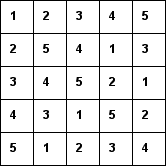
\includegraphics{./img/lat_quadrat.png}
\caption{Lateinisches Quadtrat}
\end{center}
\end{figure}

Daraus hat sich das heutige Sudoku entwickelt, das sich nicht nur bei Mathematikern großer Beliebtheit erfreut.
	\section{Die Regeln}
Diese Arbeit beschäftigt sich nur mit der meist verbreiteten Art von Sudokus. Dabei spielt man auf einem 9x9 Felder großen Spielfeld, das wiederum in neun 3x3 Felder große Blöcke eingeteilt ist. Weiter handelt es sich nur dann um ein Sudoku, wenn genau eine Lösung vorhanden ist.
Ein Sudoku gilt dann als gelöst, wenn jede Zeile, jede Spalte und jeder Block die Ziffern 1 bis 9 genau einmal enthält.\\
\begin{figure}[h]
\begin{center}
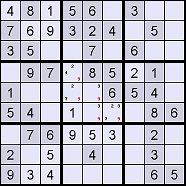
\includegraphics{./img/sudoku.jpg}
\caption{Sudoku}
\end{center}
\end{figure}
	\section{Begriffserklärung}
Ein Sudoku besteht aus 81 \textit{Feldern} oder \textit{Zellen}. In diese werden die \textit{Ziffern} oder \textit{Zahlen} eingetragen und sie bilden ein Quadrat der Größe 9x9, das \textit{Grid}. Aufgrund dieser Aufteilung hat ein Sudoku 9 \textit{Zeilen} und 9 \textit{Spalten}. Das Grid wird in 9 Unterquadrate geteilt, die jeweils 3x3 Felder groß sind. Diese werden \textit{Blöcke} genannt. Zeilen, Spalten und Blöcke werden unter dem Begriff \textit{Figur} zusammengfasst. Die Nummerierung der Blöcke erfolgt zeilenweise von links oben nach rechts unten.\\
\textit{Vorgaben} sind Zahlen, die schon von Anfang an gegeben sind.\\
In \textbf{Abbildung 2.2} sieht man im mittleren Block sogenannte \textit{Kandidaten}. Ein Kandidat ist eine Zahl, die in der Zelle noch möglich ist. Jede Zelle hat ihre eigene Liste mit Kandidaten.\\
In der Beschreibung der Lösungstechniken ist es notwendig bestimmte Felder zu betrachten. Hierzu wird eine Abkürzung verwendet, die Zeile und Spalte enthält und somit eine Zelle eindeutig indentifiziert. \textit{z2s3} meint zum Beispiel die Zelle in Zeile 2 und Spalte 3.\\
In der folgenden Abbildung sind die erläuterten Begriffe zum besseren Verständniss eingetragen.\\

\begin{figure}[h]
\begin{center}
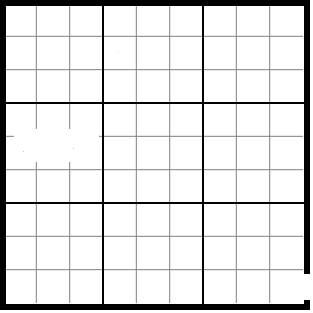
\includegraphics{./img/begriffe.png}
\caption{Begriffe}
\end{center}
\end{figure}

\chapter{Existierende Einteilungsschemata}
Für die Zuordnung eines Schwierigkeitsgrades zu einem Sudoku existieren bereits verschiedene Methoden. Die einfachsten orrientieren sich nur an Merkmalen, die auf den ersten Blick sichtbar sind, wie etwa die Anzahl der vorgegebenen Ziffern. Diese Methoden haben den Vorteil, dass das Sudoku bewertet werden kann, ohne es zu lösen. Ausserdem sind sie sehr einfach zu implementieren und auch sehr schnell. Die Genauigkeit solcher Methoden ist allerdings nicht besonders hoch, da die offensichtlichen Merkmale nicht mit einbeziehen, wie schwer das Lösen eines Sudokus ist, da es ja während der Bewertung des Sudokus nicht gelöst wird und somit dem Lösungsweg kein Schwierigkeitsgrad zugeordnet werden kann.\\
Daher ist es sinnvoll, das Sudoku bei der Bewertung zu lösen und die Schwierigkeit des Lösungsweges zu schätzen. Ein Lösungsweg besteht aus einer Reihe von Lösungsschritten. Mit jedem Schritt erfährt der Spieler mehr über das Sudoku, das bedeutet, dass er eine Ziffer einsetzen kann oder dass er ausschließt, dass eine Ziffer in einem bestimmten Feld stehen kann. Gegebenenfalls kann er mit einem Lösungsschritt sogar mehrere Ziffern in einem Feld, oder eine Ziffer in mehreren Felder ausschließen. Sehr komplexe Methoden erlauben auch den gleichzeitigen Ausschluss von mehreren Ziffern in mehreren Feldern.\\
Es gibt also verschiedene Arten von Lösungsschritten, diese haben auch eine verschiedene Schwierigkeit. Dabei entscheidend ist für diese Arbeit die vom menschlichen Spieler empfundene Schwierigkeit und nicht etwa die Komplexität der Implementierung oder die Laufzeit der Lösungsmethode auf einem Rechner, da die Bewertung später als Orrientierung für Menschen dienen soll.\\
Die Website \url{http://sudoku.soeinding.de/strategie/strategie03.php} ist ein Beispiel für ein solches Vorgehen.\\
Eine weitere Methode ist die Messung der Zeit, die menschliche Spieler zum Lösen von Sudokus brauchen. Hierbei ist das Problem, dass die Klassifikation eines Sudokus sehr lange dauert, da es erst von mehreren Spielern gelöst werden muss. Ausserdem ist die Erfahrung und damit die Spielstärke von Sudoku Spielern sher unterschiedlich und sollte in die Bewertung mit einfließen.\\
Ein Beispiel für diesen Ansatz der Klassifikation ist diese Website \url{http://sudokugarden.de/de/online/dstats}.\\
In dieser Arbeit wird versucht, ein Einteilungsschma zu finden, dass auf der Schwierigkeit des Lösungsweges beruht, aber auch offensichtliche Merkmale einbezieht.

\chapter{Lösungsmethoden}
Alle in dieser Bachelorarbeit beschriebenen Techniken sind nicht im Rahmen dieser Arbeit entwickelt worden, sondern wurden aus verschiedenen Quellen zusammengetragen. Die Beschreibung der Lösungstechniken lehnt sich an die Beschreibung der Quellen an. Teile der Beispiele wurden aus den Quellen entnommen, dies ist entsprechend gekennzeichnet.\\
Grob kann man die Techniken zum Lösen von Sudokus in zwei Kategorien einteilen. Die erste Kategorie findet Zahlen heraus, die direkt in das Sudoku eingetragen werden können. Die Techniken der zweiten Kategorie entfernen Bedingungen in einzelnen Zellen des Sudokus.
	\section{Kandidatenlisten}
\label{Kandidatenlisten}
Beim Lösen von Sudokus ist es üblich, in jedes Feld die Kandidaten einzutragen, die dort stehen können. Dabei wird vorerst nur die Sudoku Regel berücksichtigt, die besagt, dass in jeder Figure die Zahlen 1 bis 9 vorkommen müssen. Wenn in einer Zeile nun die Zahl 3 vorkommt, dann kann sie in der selben Zeile nicht nochmal vorkommen, daher kann sie aus allen Kandidatenlisten der Zellen in der selben Zeile gelöscht werden. Dasselbe gilt für Spalten und Blöcke. Immer wenn eine Ziffer in ein Feld eingetragen wird, dann muss der Spieler die Liste der Kandidaten aktualisieren.\\
Kandidatenlisten sind keine eigene Lösungstechnik, sind aber wesentlicher Bestandteil vieler Techniken.
	\newpage
\section{Full House}
\label{Full_House}
Wenn in einer Figur 8 Zahlen eingetragen sind, dann kann die Technik \textit{Full House} angewendet werden. Da in jeder Figur die Zahlen 1 bis 9 stehen müssen, kann die fehlende Zahl einfach per Ausschluss ermittelt werden.\\

\begin{figure}[h]
\begin{center}
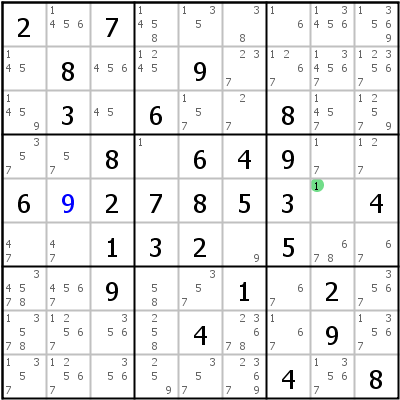
\includegraphics{./img/full_house.png}
\caption{Full House}
\end{center}
\end{figure}

In \textbf{Abbildung 3.1} fehlt in Zeile 5 nur noch eine Ziffer. Da die Zahlen 2 bis 9 bereits vorhanden sind, kann in das Feld z5s8 die Zahl 1 eingetragen werden.
	\newpage
\section{Naked Single}
\label{Naked_Single}
Bei der Technik \textit{Naked Single} werden Kandidatenlisten verwendet. Diese Technik kann angewendet werden, wenn in der Kandidatenliste einer Zelle nur noch ein Kandidat steht. Dieser Kandidat kann dann in die Zelle eingetragen werden. Das funktioniert aufgrund des Aufbaus der Kandidatenlisten. Diese enthalten zuerst alle Kandidaten und es werden immer dann Kandidaten entfernt, wenn dieser Kandidat nicht mehr als Ziffer in der Zelle stehen könnte wel er dort eine Regel verletzen würde. Wenn also nur noch ein Kandidat in der Kandidatenliste steht, dann bedeutet das, dass dieser Kandidat die einzige Ziffer zwischen 1 und 9 ist, die in der Zelle stehen kann ohne eine Regel zu verletzen.

\begin{figure}[h]
\begin{center}
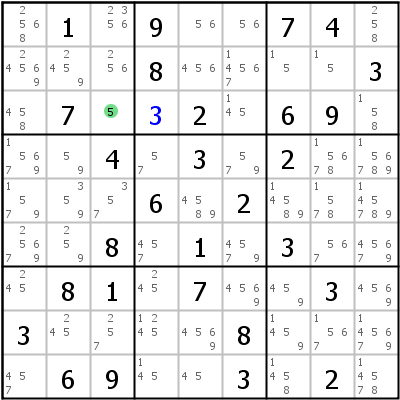
\includegraphics{./img/naked_single.png}
\caption{Naked Single}
\end{center}
\end{figure}

Im oben stehenden Beispiel \textbf{Abbildung 3.2} sieht man sofort, dass die Kandidatenliste in z3s3 nur noch einen Eintrag enthält. Dieser kann nun einfach eingetragen werden.
	\newpage
\section{Hidden Single}
Auch die Technck \textit{Hidden Single} arbeitet wieder mit Kandidatenlisten. Wenn in einer Figur eine Kandidatenliste die einzige ist, in der eine bestimmte Zahl vorkommt, dann kann diese Zahl direkt in die Zelle eingetragen werden. Wenn in dieser Zelle die Zahl nicht stünde, dann gäbe es in der Figur keine Möglichkeit mehr, dass die Zahl auftaucht und damit wäre die Sudoku Regel verletzt, nach der jede Zahl genau einmal enthalten sein muss.

\begin{figure}[h]
\begin{center}
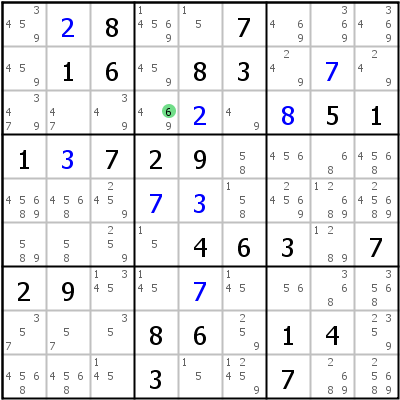
\includegraphics{./img/hidden_single.png}
\caption{Hidden Single}
\end{center}
\end{figure}

In \textbf{Abbildung 3.3} sieht man, dass die Zahl 6 in der Zeile 3 nur in z3s4 vorkommen kann. Daher kann man sie dort eintragen.

	\newpage
\section{Pointing Pair / Triple}
Bei der Technik \textit{Pointing Pair / Triple} müssen zum ersten mal die Kandidatenlisten mehrerer Felder gleichzeitig betrachtet werden, was diese Technik etwas schwerer macht. Ausserdem ist diese Technik die erste, die Kandidaten aus Kandidatenlisten entfernt und nur bedingt zum Einsetzen von Zahlen in das Sudoku führt.\\
Es werden die Kandidatenlisten in Blöcken jeweils zeilen- und spaltenweise betrachtet. Die Technik \textit{Pointing Pair / Triple}
kann angewendet werden, wenn in einem Block eine Kandidat nur in Kandidatenlisten der selben Zeile oder Spalte vorkommt. Dann kann jedes weitere vorkommen der Zahl in einer Kandidatenliste der selben Zeile oder Spalte entfernt werden. Das gilt, da die Zahl genau einmal in dem Block vorkommen muss. Da alle möglichen Vorkommen der Zahl in der selben Zeile oder Spalte liegen ist klar, dass die Zahl in dieser Zeile oder Spalte vorkommt. Da sie aber kein zweites mal in der Zeile oder Spalte vorkommen darf muss sie aus den Kandidatenlisten entfernt werden, die nicht im selben Block liegen.

\begin{figure}[h]
\begin{center}
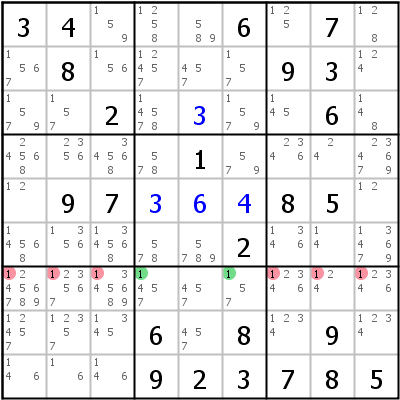
\includegraphics{./img/pointing_pair_triple.png}
\caption{Pointing Pair / Triple}
\end{center}
\end{figure}

In \textbf{Abbildung 3.4} betrachten wir Block 8. Hier ist das Vorkommen der Zahl 1 in den Kandidatenlisten auf Zeile 7 beschränkt. Wie oben beschrieben können nun alle weiteren vorkommen in der selben Zeile, die nicht in Block 8 liegen aus den Kandidatenlisten entfernt werden. Im vorliegenden Beispiel führt das allerdings nicht dazu, dass eine neue Zahl in das Sudoku eingetragen wird. Dennoch ist das Sudoku nun genauer bestimmt, da weniger Möglichkeiten übrig sind.
	\newpage
\section{Box-Line Reduction}
Die Technik \textit{Box-Line-Reduction} ist verwandt mit der Technik \textit{Pointing Pair / Triple}. Hier wird das Sudoku zeilen- und spaltenweise betrachtet. Ist das Vorkommen einer Zahl in den Kandidatenlisten auf einen Block beschränkt, dann kann jedes weitere Vorkommen der Zahl aus den Kandidatenlisten der Zellen des selben Blocks gestrichen werden, die nicht in der Zeile oder Spalte liegen. Die Begründung dafür ist ähnlich der Begründung bei \textit{Pointing Pair / Triple}. Da die Zahlen 1 bis 9 jeweils genau einmal in der Zeile oder Spalte vorkommen müssen und dieses Vorkommen auf einen Block beschränkt ist, ist klar, dass die Zahl letztendlich in diesem Block vorkommt und zwar in der gefundenen Zeile oder Spalte. Die Zahl kann aber nicht zweimal in dem Block vorkommen, daher kann sie aus den Kandidatenlisten des Blocks gelöscht werden, deren Zellen sich nicht in der Reihe oder Spalte befinden.

\begin{figure}[h]
\begin{center}
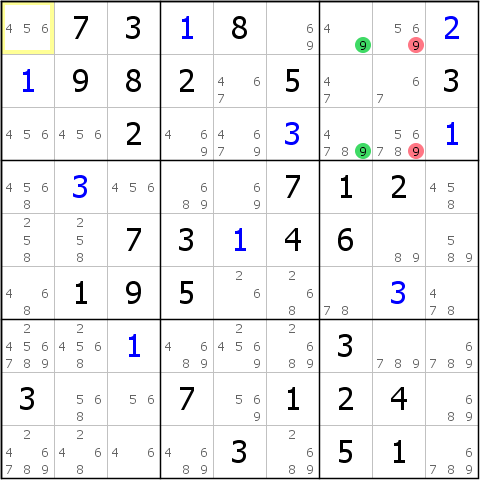
\includegraphics{./img/box_line_reduction.png}
\caption{Box-Line Reduction}
\end{center}
\end{figure}

Wir betrachten Spalte 6 in \textbf{Abbildung 3.5}. Hier sieht man, dass das Vorkommen der Zahl 4 in dieser Spalte auf Block 2, den oberen Block, beschränkt ist. Anhand dieser Spalte sieht man also, dass die Zahl 4 entweder in z2s6 oder in z3s6 steht, also in jedem Fall in Block 2. Daher kann die Zahl 4 aus den Kandidatenlisten der anderen Zellen in Block 2 gestrichen werden.

	\newpage
\section{Naked Subset}
Die Technik \textit{Naked Subset} ist ein Überbegriff für die Techniken \textit{Naked Pair}, \textit{Naked Triple} und \textit{Naked Quadruple}. Alle Techniken Arbeiten nach dem selben Prinzip, der Unterschied liegt in der Anzahl der verwendeten Kandidatenlisten. Bei \textit{NakedSubsets} sucht man nach Paaren, Tripeln oder Quadrupeln von Zellen in Figuren, nach Kandidatenlisten einer bestimmten Eigenschaft. Die Vereinigung der Listen muss eine bestimmte Anzahl Elemente enthalten. Bei Paaren sind das zwei, bei Tripeln drei und bei Quadrupeln vier Einträge in den Kandidatenlisten.\\
Findet man zum Beispiel ein Paar, das nur noch die selben beiden Zahlen enthalten kann dann ist klar, dass keine der Zahlen anderswo in der Figur stehen kann, da sonst für eine der Zellen keine Zahl mehr übrig bleibt. Daher können die beiden Zahlen dann aus den Kandidatenlisten aller anderen Zahlen aus der Figur entfernt werden.
Die Begründung für Tripel und Quadrupel ist analog.\\
Es ist nicht nötig nach mehr als Quadrupeln zu suchen, da für jedes Naked Quintupel ein Hidden Quadrupel existiert.

\begin{figure}[h]
\begin{center}
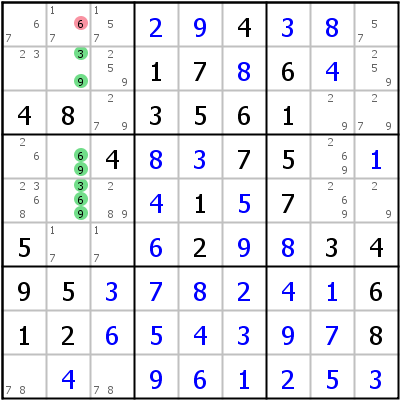
\includegraphics{./img/naked_subset.png}
\caption{Naked Subset - Naked Triple}
\end{center}
\end{figure}

In \textbf{Abbildung 3.6} findet man das \textit{Naked Subset}, bei dem es sich um ein \textit{Naked Triple} handelt, in Spalte 2. Hier hat die Vereinigung der Kandidatenlisten der Zellen z2s2, z4s2 und z5s2 genau drei Einträge: 3, 6 und 9. Es gibt offensichtlich keine andere Möglichkeit, als die drei Zahlen auf diese Felder zu verteilen, Demnach können sie in der Reihe sonst nicht vorkommen und können aus den Kandidatenlisten der anderen Zellen entfernt werden.

	\newpage
\section{Hidden Subset}
Analog zu den \textit{Naked Subset}-Techniken ist auch \textit{Hidden Subset} ein Sammelbegriff. Er beinhaltet die Techniken \textit{Hidden Pair}, \textit{Hidden Triple} und \textit{Hidden Quadruple}. Auch hier ändert sich nur die Anzahl der betrachteten Kandidatenlisten. Hier soll exemplarisch die Technik \textit{Hidden Tuple} erklärt werden, im folgenden Beispiel wird dann die Technik \textit{Hidden Quadruple} angewendet.\\
Wenn man in einer Figur zwei Zahlen findet, die ausschließlich in den zwei gleichen Zellen vorkommen können, dann müssen diese beiden Zahlen in die beiden Zellen gesetzt werden. Daher kann man alle anderen Kandidaten in den Zellen von der Kandidatenliste streichen.

\begin{figure}[h]
\begin{center}
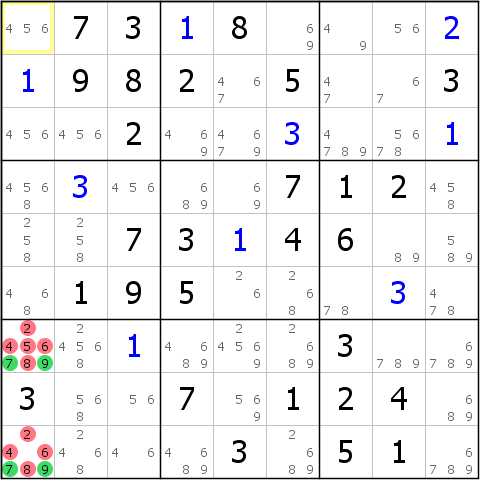
\includegraphics{./img/hidden_subset.png}
\caption{Hidden Subset - Hidden Quadruple}
\end{center}
\end{figure}

In \textbf{Abbildung 3.7} betrachten wir den Block 8 und in diesem Block die Zellen z6s5, z6s6, z7s5 und z7s6. Nur in diesen Zellen können die Zahlen 4, 5, 6 und 8 vorkommen. Da wir diese vier Zahlen nun auf die vier Zellen verteilen müssen gibt es dort keinen Platz mehr für andere Zahlen. Diese können also aus den Kandidatenlisten entfernt werden.

	\newpage
\section{Fish}
\label{Fish}
Die \textit{Fish} Methoden sind ein Sammelbegriff für eine ganze Grupppe von Methoden, die alle nach dem gleichen Prinzip arbeiten. Wie echte Fische hat dieses Prinzip eine sehr große Anzahl Unterarten hervorgebracht. Kleine Fische wie zum Beispiel X-Wing sind von geübten Sudoku Spielern noch zu finden, wenn die Fische allerdings größer werden, dann sind sie nur noch mit sehr hohem Aufwand manuell zu finden und daher eher zur Verarbeitung mit dem Computer gedacht. \\
Auf einer Internetseite, die sich unter anderem mit den Lösungsmethoden für Sudokus befasst, findet sich die folgende Erklärung zur Funktionsweise von Fischen.

\begin{quote}[...] Man suche eine bestimmte Anzahl von Häusern, die sich nicht überschneiden. Diese Häuser werden als Base-Sets (Basismengen) bezeichnet (Set wird hier synonym für Haus verwendet), die in diesen Häusern enthaltenen Kandidaten sind die Basiskandidaten. Nicht überschneiden bedeutet hier, dass kein Basiskandidat in mehr als einem Haus enthalten sein darf, die Häuser selbst dürfen sich schon überlappen. Nun suche man eine gleiche Anzahl an sich nicht überschneidenden Häusern, die alle Basiskandidaten abdecken (engl.: cover). Diese neuen Häuser sind die Cover-Sets, sie enthalten die Coverkandidaten. Wenn eine solche Kombination existiert, können alle Coverkandidaten gelöscht werden, die nicht gleichzeitig Basiskandidaten sind.
\footnote{Quelle: \url{http://hodoku.sourceforge.net/de/tech_fishg.php}}
\footnote{Häuser stehen hier für Figuren}
\end{quote}
		\newpage
\subsection{Basic Fish}
\label{X-Wing}
Die Techniken \textit{X-Wing}, \textit{Swordfish} und \textit{Jellyfish} sind die einfachsten Unterarten der Fische. Sie funktionieren nach dem selben Prinzip, nur dass eine unterschiedliche Anzahl an Figuren betrachtet wird, ähnlich zu \textit{Naked Subset} und \textit{Hidden Subset}. Hier wird stellvertretend die Technik \textit{X-Wing} erklärt und am Beispiel gezeigt.\\
Dazu sucht man zwei Spalten oder Zeilen, die ausschließlich in den selben zwei Zellen einen bestimmten Kandidaten, die Fischziffer, beinhalten. Nun kann man aus dem jeweils anderen Paar von Figuren (Spalte oder Zeile), deren Position durch die zwei gefundenen Zellen festgelegt wird, alle Fischziffern löschen, die nicht gleichzeitig in einer der zuerst ausgesuchten Figuren liegen.\\
Da die Fischziffer in den beiden zuert ausgesuchten Figuren nur an jeweils zwei Stellen liegen kann und diese sich paarweise gegeinseitig ausschließen ist klar, dass jedes Vorkommen der Fischziffer in den zuletzt ausgesuchten Figuren in der Überschneidung mit den ersten Figuren liegen muss.

\begin{figure}[h]
\begin{center}
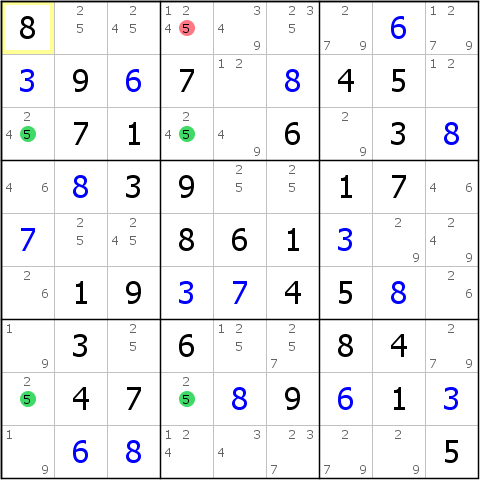
\includegraphics{./img/x_wing.png}
\caption{Basic Fish - X-Wing}
\end{center}
\end{figure}

Ein Beispiel für die Technik \textit{X-Wing} findet sich in \textbf{Abbildung 3.8}. Hier wurden als erste Figuren die Zeilen 2 und 5 gewählt. Diese enthalten die Fischziffer 5 nur an den Stellen 5 und 8. Wichtig ist, dass es in den beiden Zeilen die gleichen Positionen sind. Da die Ziffer 5 und Zeile 2 nur an den Positionen 5 und 8 stehen kann werden beiden Fälle nun gtrennt betrachtet. Steht in z2s5 die Ziffer 5, dann muss sie auch in z5s8 stehen, da sonst die Zeile 5 die Ziffer 5 nicht enthalten würde. Umgekehrt gilt:Steht in z2s8 die Ziffer 5, dann muss sie auch in z5s5 stehen. In jedem der beiden möglichen Fälle gilt, dass sowohl in Spalte 5 als auch in Spalte 8 die Ziffer 5 vorkommt und zwar in den Zeilen 2 und 5. Daher kann aus allen anderen Zellen der Spalten die Fishziffer 5 gelöcht werden, falls sie in den Kandidatenlisten vorhanden ist.
	\newpage
\section{Single Digit Patterns}
\textit{Single Digit Patterns} ist ein Oberbegriff für Techniken, denen allen gemeinsam ist, dass sie nur eine Ziffer betrachten. Die Techniken textit{Skyscarper} und \textit{2-String-Kite} sind Unterarten der Technik \textit{Turbot Fish}, die aber für den Menschen einfacher zu finden sind. Da der Schwierigkeitsgrad des Sudokus für Menschen bewertet werden soll, werden sie hier mit aufgelistet und auch im Programm verwendet.
		\subsection{Skyscarper}
\label{Skyscarper}
Die Technik \textit{Skyscarper} bedeutet übersetzt Wolkenkratzer und leitet sich von der Anordnung der betrachteten Ziffern ab. Gesucht werden zwei Zeilen oder Spalten, in deren Kandidatenlisten die Ziffer jeweils noch genau zwei mal auftaucht. Wenn nun zwei der Kandidaten in der selben anderen Figur (Spalte oder Zeile) sind, dann hat man einen Wolkenkratzer gefunden. Die beiden Zahlen, die in der selben anderen Figur sind, bilden das Fundament des Woleknkratzers, sie schließen sich gegenseitig aus. Das bedeutet wiederum, dass eine der beiden anderen gefundenen Ziffern dort stehen muss. Daher können alle Kandidaten, die von beiden Ziffern ausgeschlossen werden, aus den Kandidatenlisten gelöscht werden.	

\begin{figure}[h]
\begin{center}
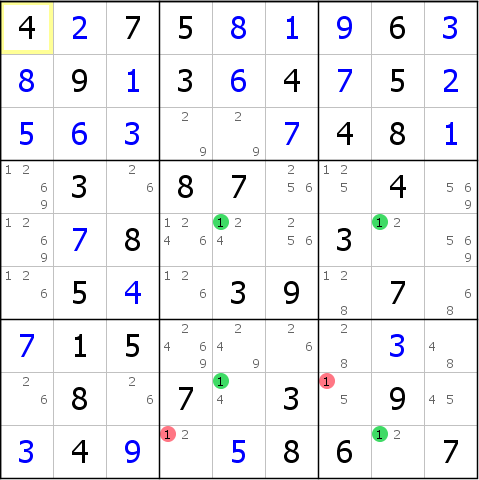
\includegraphics{./img/skyscarper.png}
\caption{Skyscarper}
\end{center}
\end{figure}

In \textbf{Abbildung 3.9} betrachten wir die Spalten 6 und 9. Hier sind die Bedingungen für den Wolkenkratzer erfüllt, da in jeder Spalte die Ziffer 1 jeweils genau zwei mal vorkommt und sie in jeder Spalte an Position 5 auftaucht. Für das Feld z3s9 gibt es nun zwei Möglichkeiten. Entweder die Ziffer 1 steht in diesem Feld oder nicht. Diese beiden Möglichkeiten werden nun separat betrachtet. Wenn die Ziffer 1 in Feld z3s9 steht, dann schließt das bereits alle rot markierten Zahlen aus. Für den Fall, dass die Ziffer 1 nicht in z3s9 steht, muss sie in z5s9 stehen, das geht aus der Bedingung des Wolkenkratzers hervor. Da sich nun z5s9 und z5s6 laut Bedingung in der selben Zeile befinden, kann die Ziffer 1 nicht in z5s6 vorkommen. Deshalb muss sie in z1s6 stehen, wo sie alle rot markierten Felder ausschließt.
		\newpage
\subsection{2-String Kite}
Die Technik \textit{2-String-Kite} wird auch Paierdrache genannt, was sich, wie beim Wolkenkratzer, aus der Anordnung der Zahlen ableitet. Auch hier wird nur eine einzige Ziffer betrachtet. Gesucht werden eine Zeile und eine Spalte, die nur noch zwei Kandidaten der betrachteten Ziffer enthalten, so dass ein Kandidat der Spalte und ein Kandidat der Zeile im selben Block liegen. Die Zeile und die Spalte nennt man die \textit{Schnüre} des Drachens. Die Enden der Schnüre liegen im gleichen Block, die Position des Anfangs ist relevant für das Löschen des Kandidaten. Gelöscht werden kann nämlich der Kandidat in der Zelle, die von beiden Anfängen der Schnüre ausgeschlossen wird. Das kommt zustande, da die betrachtete Ziffer in jedem Fall am Anfang einer der beiden Schnüre stehen muss.

\begin{figure}[h]
\begin{center}
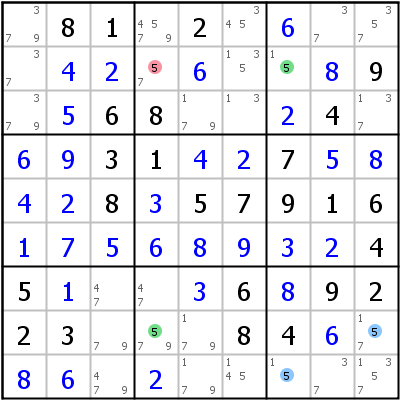
\includegraphics{./img/2stringkite.png}
\caption{2-String-Kite}
\end{center}
\end{figure}

\textbf{Abbildung 3.10} zeigt einen \textit{2-String-Kite}. Betrachtet wird die Ziffer 5, Zeile 8 und Spalte 7 fungieren als Schnüre des Drachen. In z2s7 betrachten wir zwei Fälle: Entweder die Ziffer 5 steht dort oder sie steht dort nicht. Für den ersten Fall gilt, dass dann die rot markierte Ziffer in z2s4 ausgeschlossen ist. Der zweite Fall ist etwas komplizierter. Wenn die Ziffer 5 nicht in z2s7 steht, dann muss sie an der einzig anderen möglichen Position der Spalte stehen, nämlich in z9s7. Daher kann sie nicht in z8s9 stehen, da diese Felder im selben Block liegen. Da in Zeile 8 auch nur noch zwei Kandidaten für die Ziffer 5 übrig waren, muss sie in z8s4 stehen, wi sie z2s4 ausschließt. In jedem der Fälle kann also die Ziffer 5 nicht in z2s4 stehen und daher kann sie dort gelöscht werden.
		\newpage
\subsection{Turbot Fish}
Wie auch bei den vorherigen \textit{Single Digit Patterns} wird auch beim \textit{Turbot Fish} nur eine Ziffer betrachtet. Gesucht wird eine Kette, die vier Ziffern lang ist, so dass Anfang und Ende eines Kettenglieds in einer gemeinsamen Figur liegen. Wichtig ist dabei, dass im ersten und dritten gemeinsamen Figur die beiden betrachteten Kandidaten die einzigen verbliebenen  sind. Da die Kette vier Glieder lang ist, muss entweder der Anfang oder das Ende der Kette wahr sein, daher können die Kandidaten gelöscht werden, die von beiden Feldern ausgeschlossen werden.

\begin{figure}[h]
\begin{center}
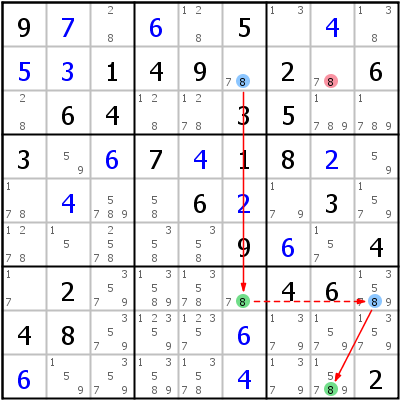
\includegraphics{./img/turbot_fish.png}
\caption{Turbot Fish}
\end{center}
\end{figure}

In der obigen \textbf{Abbildung 3.11} beginnt die Kette der Ziffer 8 im Feld z2s6. In der selben Spalte befindet sich die zweite Ziffer in z7s6, sie ist dort der einzige weitere Kandidat der Ziffer 8, was Voraussetzung für den Turbot Fish ist, da es sich hier um das erste Glied handelt. Die nächste Ziffer liegt in der gleichen Zeile, z7s9. Die letzte Ziffer befindet sich im selben Block wie auch ihr Vorgänger, in z9s8, und auch sie ist hier der einzige weitere Kandidat für diese Ziffer. Wir betrachten zwei Fälle: die Ziffer 8 steht in z2s6 oder sie steht dort nicht. Im ersten Fall kann der rot markierte Kandidat in z2s8 gelöscht werden, da er direkt ausgeschlossen wird. Wenn die 8 dort nicht steht, dann muss sie in z7s6 stehen, da das der einzige andere Kandidat in der Zeile ist. Darum kann die 8 dann nicht in z7s9 stehen. Daraus folgt, dass sie in z9s8 stehen muss, was dann im zweiten Fall die Ziffer 8 in z2s8 ausschließt, womit diese dort in jedem Fall nicht stehen kann.
		\newpage
\subsection{Empty Rectangle}
Für die Technik \textit{Empty Rectangle} gilt das selbe wie für alle \textit{Single Digit Patterns}, es wird nur eine Ziffer betrachtet und der Name leitet sich aus der Form der Anordnung der Ziffern ab. Um ein \textit{Empty Rectangle} zu finden, wird ein Block gesucht, in dem ein Kandidat ausschließlich noch in einer Zeile und in einer Spalte vorkommen kann. Dann bilden die verbliebenen Kandidaten eine Ecke eines \textit{Empty Rectangles}.

\begin{figure}[h]
\begin{center}
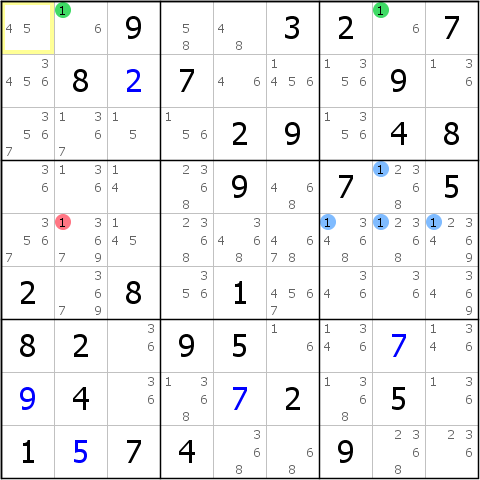
\includegraphics{./img/empty_rectangle.png}
\caption{Empty Rectangle}
\end{center}
\end{figure}

In \textbf{Abbildung 3.12} sehen wir ein \textit{Empty Rectangle}, das von Block 5 ausgeht. Die verbleibenden Kandidaten der Ziffer 1 können hier nur noch in Zeile 4 und Spalte 5 stehen. Wenn wir Zeile 7 betrachten, dann sehen wir, dass die Ziffer 1 hier nur noch an zwei Positionen stehen kann, nämlich an der fünften und an der neuten. Wir betrachten nun diese beiden Fälle getrennt. Wenn die Ziffer 1 in z7s9 steht, dann ist die Ziffer 1 in z4s9 direkt ausgeschlossen. Wenn sie in z7s5 steht, dann kann sie in Block 5 nur noch an einer Position stehen, nämlich z4s6. Auch in diesem Fall ist die Ziffer 1 dann im Feld z4s9 ausgeschlossen. Daher kann sie dort als Kandidat gelöscht werden.
	\newpage
\section{Wings}
		\subsection{XY-Wing}
Die Technik \textit{XY-Wing} wird manchmal auch nur \textit{Y-Wing} genannt, da sie aussieht wie ein \textit{X-Wing} (siehe Kapitel \ref{X-Wing}) nur mit drei Ecken. Zuerst sucht man eine Zelle, in der nur noch 2 Kandidaten verblieben sind. Diese Kandidaten nennt man dann x und y. Daher kommt der im Allgemeinen bekanntere Name der Strategie. Im nächsten Schritt sucht man nun eine Zelle, die in einer gemeinsamen Figur mit der ersten Zelle liegt und auch nur noch 2 Kanididaten der Form hat, dass einer der Kandidaten dem x aus der ersten Zelle entspricht und der zweite Kandidat ungleich dem y ist. dieser wird nun z genannt. Anschließend sucht man eine dritte Zelle mit nur noch zwei verbliebenen Kandidaten, die ebenfalls in einer gemeinsamen Figur mit der ersten Zelle liegt, aber nicht in der selben wie die zweite gefundene Zelle. Wenn diese Zelle nun die Kandidaten y und z enthält, dann hat man einen \textit{XY-Wing} gefunden. Gelöscht werden kann nun der Kandidat z aus der Zelle, die von der zweiten und dritten Zelle ausgeschlossen wird. Das funktioniert, da in der ersten Zelle entweder x oder y steht. Wenn in der ersten Zelle x steht, dann steht in der zweiten Zelle z, da dort nur x und z stehen kann, x aber durch die erste Zelle ausgeschlossen wird. Wenn in der ersten Zelle aber y steht, dann muss in der dritten Zelle z stehen, da dort nur y und z stehen können und y ausgeschlossen wird. Daher steht in einer der beiden Zellen z und alle Kandidaten von z, die durch beide Felder ausgeschlossen werden, können gelöscht werden.

\begin{figure}[h]
\begin{center}
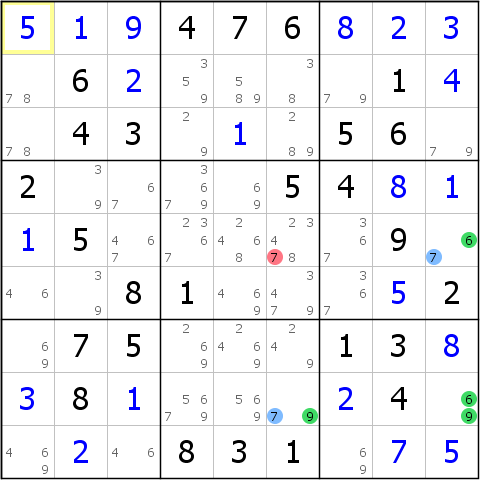
\includegraphics{./img/XY_Wing.png}
\caption{XY-Wing}
\end{center}
\end{figure}

In der obigen \textbf{Abbildung 3.13} stehen in z1s3 die Kandidaten 5 für x und 7 für x. In Zelle z1s6 stehen 5 für x und 2 für z. in z2s1 stehen 7 für y und 2 für z. Wenn in z1s3 die Ziffer 5 steht, dann muss in z1s6 die Ziffer 2 stehen und den Kanididaten 2 in z2s6 ausschließen. Wenn in z1s3 die Ziffer 7 steht, dann steht in z2s1 die Ziffer 2 und schließt ebenfalls die Ziffer 2 in z2s6 aus. Somit kann diese dort in keinem der beiden Fälle stehen und kann gelöscht werden.
		\newpage
\subsection{XYZ-Wing}
Bei der Technik \textit{XYZ-Wing} handelt ies sich um eine erweiterte Version der Technik \textit{XY-Wing}. Zusätzlich zu den Kandidaten x und y steht hier in der ersten Zelle noch der Kandidat z, der Rest ändert sich nicht. Statt zwei Fällen werden hier drei Fälle betrachtet. Wenn der Kandidat x in der ersten Zelle steht, dannn bleibt die Argumentation wie beim \textit{XY-Wing}. Das selbe gilt für den Fall, dass der Kandidat y in der ersten Zelle steht. Im dritten Fall steht der Kandidat z in der ersten Zelle. In diesem Fall würde er alle Kandidaten ausschließen, die von dort aus direkt auschgeschlossen werden. Daher können alle Kandidaten der Ziffer z gelöscht werden, die von allen drei Zellen ausgeschlossen werden.

\begin{figure}[h]
\begin{center}
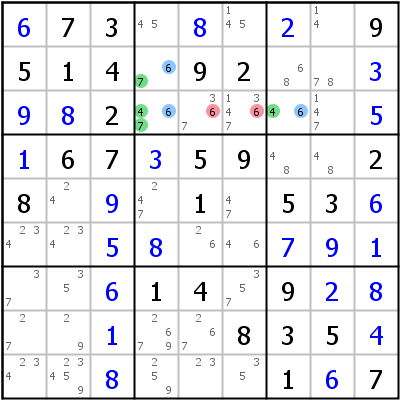
\includegraphics{./img/XYZ_Wing.png}
\caption{XYZ-Wing}
\end{center}
\end{figure}

In \textbf{Abbildung 3.14} sieht man einen \textit{XYZ-Wing}, dessen erste Zelle z3s4 ist. Hier stehen die Kandidaten 4 für x, 7 für y und 6 für z. Bei z3s7 findet man die zweite Zelle mit den Kandidaten 4 und 6, also x und z. Die dritte Zelle ist z2s4, sie enthält die Kandidaten 6 und 7 und damit y und z. Wenn die Ziffer 4 ind z3s4 steht, dann muss in z3s6 die Ziffer 6 stehen und damit sind die rot markierten Kandidaten ausgeschlossen. Wenn in z3s4 die Ziffer 7 steht, dann muss in z2s4 die Ziffer 6 stehen und auch in diesem Fall sind die rot markierten Kandidaten ausgeschlossen. Wenn in z3s4 die Ziffer 6 steht, dann sind ebenfalls die rot markierten Kandidaten ausgschlossen. Somit können sie in jedem der möglichen Fälle ausgeschlossen werden und werden daher gelöscht.
		\newpage
\subsection{W-Wing}
Die Technik \textit{W-Wing} ist die letzte und schwierigste Technik der Wings. Hierbei werden immer zwei Ziffern betrachtet. Zuerst sucht man eine Zelle, in der nur noch zwei Kandidaten x und y möglich sind. Nun wird eine Figur gesucht, in der der Kandidat x nur noch zwei mal vorkommen kann und eines der möglichen Vorkommen von der ersten Zelle ausgeschlossen würde. Im letzten Schritt sucht man eine Zelle, die wieder ausschließlich die Kandidaten x und y enthält und die das andere mögliche Vorkommen der Ziffer x in der zuvor gefundenen Figur ausschließen würde. Findet man eine solche Konstelation, dann handelt es sich um einen \textit{W-Wing}. Gelöscht werden können die  Kandidaten y, die von beiden Zellen gleichzeitig ausgeschlossen werden, da der Kandidat y entweder in der ersten oder in der zweiten gefundenen Zelle stehen muss.

\begin{figure}[h]
\begin{center}
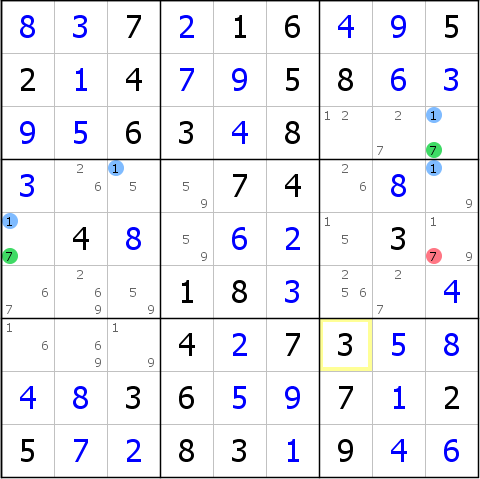
\includegraphics{./img/W_Wing.png}
\caption{W-Wing}
\end{center}
\end{figure}

In \textbf{Abbildung 3.15} betrachten wir zuerst z8s9. Hier finden wir die Ziffer 9 für x und 5 für y. Die gesuchte Figur ist Spalte 8, da hier der Kandidat 9 nur noch zwei mal vorkommen kann und eines der Vorkommen von z8s9 ausgeschlossen wird.
Das andere Vorkommen wird von z4s4 ausgeschlossen. In dieser Zelle befinden sich ausserdem nur noch die Kandidaten x und y. Damit ist die Bedingung für den \textit{W-Wing} erfüllt und der rot markierte Kandidat kann gelöscht werden. Wir betrachten zwei Fälle, entweder die Ziffer 5 steht in z8s9 oder nicht. Im ersten Fall würde der rot markierte Kandidat direkt ausgeschlossen werden. Wenn die Ziffer 5 nicht in z8s9 steht, dann steht dort die Ziffer 9. Damit kann die in Spalte 8 nur noch an Position 4 stehen und damit muss in z4s4 die Ziffer 5 stehen, was wiederum den rot markierten Kandidaten ausschließt. In keinem der Fälle kann der Kandidat dort stehen und wird daher gelöscht..t
	\newpage
\section{Sue de Coq}
Die Technik \textit{Sue de Coq} wurde ursprünglich unter dem Namen \textit{Two-Sector Disjoint Subsets} in einem Forum\footnote{\url{http://forum.enjoysudoku.com/two-sector-disjoint-subsets-t2033.html}} vorgestellt. Anderen Benutzern des Forums war dieser Name zu umständlich und sie begannen die Strategie als \textit{Sue de Coq} zu bezeichnen, dem Benutzernamen des Vorstellers.\\
Um die Technik anzuwenden sucht man zuerst zwei oder drei Zellen in einem Block, die in der selben Reihe oder Spalte liegen. Die Vereinigung der Kandidatenlisten muss dabei bei zwei Zellen vier Kandidaten enthalten und bei drei Zellen müssen fünf Kandidaten vorhanden sein. Nun sucht man zusätzlich eine Zelle im selben Block, die ausschließlich zwei Kandidaten der Vereinigung enthält. Eine solche Zelle sucht man auch in der Reihe oder Spalte, in der die ersten Zellen liegen. Die Schnittmenge der Kandidatenlisten der beiden zusätzlichen Zellen muss leer sein. \\
Die Kandidaten aus der zusätzlichen Zelle in der Reihe können nun aus allen unbeteiligten Zellen der Reihe gelöscht werden.  Das gilt ebenfalls für die Kandidaten der zusätzlichen Zelle des Blocks, diese können aus allen unbeteiligten Zellen des Blocks entfernt werden.\\

\begin{figure}[h]
\begin{center}
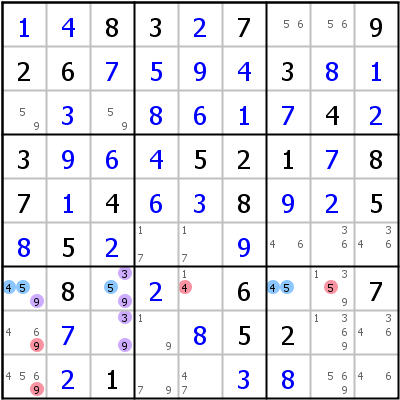
\includegraphics{./img/Sue_de_Coq.png}
\caption{Sue de Coq}
\end{center}
\end{figure}

In Abbildung \textbf{3.16} sieht man einen \textit{Sue de Coq} mit den zwei Basiszellen z7s1 und z7s3. Diese liegen im Block 7 in der selben Zeile. Die Vereinigung der Kandidaten enthält die Ziffern 3, 4, 5 und 9. Die zusätzliche Zelle in der Zeile ist z7s7. Sie enthält die Kandidaten 4 und 5 die Teilmenge der vorherigen Vereinigung ist. Die zusätzliche Zelle im Block 7 ist z8s3. Diese enthält die Kandidaten 3 und 9, die ebenfalls Teilmenge der Vereinigung ist. der Schnitt der Kandidatenlisten der zusätzlichen Zellen ist leer. Damit sind alle Bedingungen für den \textit{Sue de Coq} erfüllt und die rot markierten Kandidaten können gelöscht werden.
	\newpage
\section{Coloring}
	\newpage
\section{Almost Locked Set}
Ein \textit{Locked Set} bezeichnet eine Gruppe von n ungelösten Zellen, deren Vereinigung der Kandidatenlisten nur noch n Kandidaten enthält. Das erlaubt das Entfernen aller Kandidaten aus den anderen Zellen der Figur, die in der Vereinugung der Kandidatenlisten vorkommen.\\
Ein \textit{Almost Locked Set} hat $n+1$ Kandidaten und ist daher einzeln nicht zu gebrauchen. Man kann allerdings Informationen erhalten, indem man zwei \textit{Almost Locked Sets} kombiniert. Dazu müssen sie mindestens einen gemeinsamen Kandidaten haben für den zusätzlich gilt, dass alle Instanzen des Kandidaten in ALS 1 alle Instanzen des Kandidaten in ALS 2 sehen können. Dieser Kandidat kann dann nur einmal in beiden ALS gesetzt werden, da sich alle Instanzen gegenseitig ausschließen.
		\newpage
\subsection{ALS XZ}
Die Technik \textit{ALS XZ} ist die einfachste Unterart der \textit{Almost Lockes Sets}. Man sucht zwei \textit{ALS} mit einem \textit{RCC}. Dieser wird X genannt. Wenn beide \textit{ALS} noch einen gemeinsamen Kandidaten Z besitzen, der kein \textit{RCC} ist, dann kann Z aus allen Zellen gelöscht werden, die nicht zum \textit{ALS} gehören und die alle Instanzen von Z in beiden \textit{ALS} sehen. Das funktioniert, da durch X ein \textit{ALS} zum \textit{Locked Set} wird. Da in beiden \textit{ALS} die Ziffer Z vorkommt wird diese auf ein \textit{ALS} beschränkt. Das bedeutet, dass Z in genau einem \textit{ALS} vorkommt und daher können alle Kandidaten gelöscht werden, die von allen Instanzen gesehen werden.

\begin{figure}[h]
\begin{center}
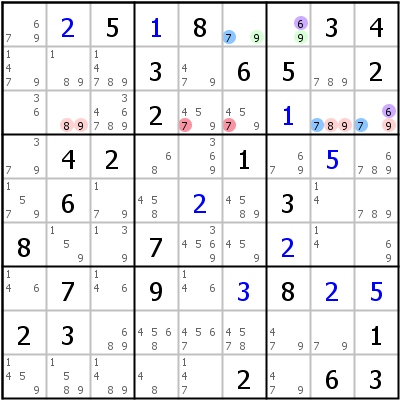
\includegraphics{./img/ALS_XZ.png}
\caption{ALS XZ}
\end{center}
\end{figure}

In \textbf{Abbildung 4.18} sehen wir die beiden \textit{ALS} einmal in Zeile 1 Spalte 6 und 7 mit den Kandidaten 6, 7 und 9 und das zweite in Zeile 3 Spalte 2, 8 und 9 mit den Kandidaten 6, 7, 8 und 9. Der \textit{RCC} ist hier die Ziffer 6, da alle Instanzen in beiden \textit{ALS} in Block 3 liegen. Ausserdem kommt in beiden \textit{ALS} die Ziffer 7 vor, die aber kein \textit{RCC} ist, da sich zum Beispiel z1s6 und z3s9 nicht sehen können. Nun können alle Zellen die Ziffr 7 von ihren Kandidatenlisten, die alle Instanzen der Ziffer 7 in beiden \textit{ALS} sehen, was z3s5 und z3s6 sind.
		\newpage
\subsection{ALS XY Wing}
		\newpage
\subsection{ALS Chain}

\chapter{Klassifikation}
Unter einer Klassifikation versteht man in der Informatik das Einteilen von Objekten in vorher festgelegte Klassen. Diese Einteilung wird von einem Algorithmus durchgeführt, der anhand von festgelegten Merkmalen jedem Objekt eine Klasse zuordnet. Einen solchen Algorithmus nennt man Klassifikator. Um die Qualität eines Klassifikators zu analysieren gibt es verschiedene Metriken.
\begin{itemize}
\item Accuracy - Die Anzahl der richtig zugeordneten Klassen
\item Recall - Der Anteil der positiven Beispiele, die auch positiv klassifiziert wurden
\item Precision - Der Anteil der positiv klassifizierten Beispiele, die auch positiv sind
\end{itemize}
Ein Klassifikator benötigt vor der Phase der Klassifikation aber zunächst einmal eine Trainigsphase, in der er anhand von Beispielen lernt. Mit dem erlenten Wissen wird anschließend die Einteilung in die Klassen vorgenommen.\\
Es gibt viele verschiedene Ansätze für Klassifikatoren, von denen die wichtigsten in einem open source Framework implementiert sind. Dieses Framework heisst Weka\footnote{\url{http://www.cs.waikato.ac.nz/ml/weka/index.html}} und wurde im praktischen Teil dieser Bachelorthesis verwendet.\\
Weka arbeitet unter anderem mit dem .arff\footnote{\url{http://weka.wikispaces.com/ARFF}} Format. In einer .arff Datei befindet sich neben den Metadaten hauptsächlich eine Sammlung von Featurevektoren. Jeder Featurevektor beschreibt ein zu klassifizierendes Objekt. Ein Eintrag in einem Featurevektor beschreibt eine Eigenschaft des beschriebenen Objekts. Das könnte bei Fahrzeugen zum Beispiel die Anzahl der Reifen sein. Bezogen auf Sudokus bedeutet das, dass jedes Sudoku durch einen Featurevektor beschrieben wird. Jede zur Klassifikation verwendete Eigenschaft eines Sudokus ist dann ein Wert im entsprechenden Featurevektor. Die Schwierigkeitsgrade der Sudokus sind die vorgegebenen Klassen.\\
Jeder Klassifikator in Weka hat als Eingabe eine Liste von Featurevektoren. Möchte man also das Zuordnen von Sudokus zu Schwierigkeitsgraden mit Weka realisieren, dann muss eine Methode entwickelt werden, die aus einem gegebenen Sudoku einen Featurevektor extrahiert.\\
Bei der Klassifikation wird ein Verfahren angewendet, das als \textit{cross validation} bekannt ist und auch von Weka zur Verfügung gestellt wird. Dabei werden die Daten in eine vorgegebene Anzahl gleich großer Folds eingeteilt. Ein Fold ist eine Sammlung von Featurevektoren. Wenn die Einteilung in k Folds erfolgt ist, dann wird der Klassifikator k mal ausgewertet, einmal mit jedem Fold.\\
Die Qualität der resultierenden Klassifikation ist sehr stark von der Wahl der Einträge des Featurevektors abhängig. Daher lag das Hauptaugenmerk dieser Bachelorarbeit auf dem Herausarbeiten der passenden Einträge für den Featurevektor, der das Sudoku beschreibt. Später wird aber auch auf die Wahl des Klassifikators und die Optimierung der Parameter eingegangen.\\

\chapter{Trainingsdaten}
Um fundierte Aussagen über die Qualität der Klassifikation treffen zu können, wird eine große Menge an Trainingsdaten benötigt. Diese müssen bereits vollständig in Schwierigkeitsstufen eingeteilt worden sein. Das ist nötig, da der Klassifikator eine Schwierigkeitsstufe zuordnet und die Qualität der Zuordnung evaluiert werden soll. Um also festzustellen, ob der Klassifikator die richtige Klasse zugeordnet hat muss diese bekannt sein.\\
Kostenlose und frei verfügbare Sudokus in digitaler Form mit definiertem Schwierigkeitsgrad lassen sich nicht leicht finden. Daher habe ich bei einigen großen Zeitungen, aus deren Websites Sudokus zu finden waren, nachgefragt, ob es möglich ist, ihre Sudokusammlungen zur Verfügung zu stellen. Die Anfragen wurden aber leider abgelehnt. Auf eine Anfrage an die Website \url{http://sudoku.soeinding.de/} wurden von sieben Schwierigkeitsgraden jeweils 32 Sudokus bereitgestellt. Da diese Trainigsdaten nicht ausreichten wurden mit dem open source Programm Hodoku\footnote{\url{http://hodoku.sourceforge.net/de/index.php}} jeweils 1000 Sudokus von fünf unterschiedlichen Schwierigkeitsgraden generiert.\\
Wie schon an der Anzahl der Schwierigkeitsstufen zu erkennen ist, unterscheiden sich die Skalen der beiden Quellen. Daher konnten die Sudokus nicht gemeinsam klassifiziert werden. Auch war es nicht möglich, eine Quelle als Trainingsdaten für den Klassifikator zu verwenden um ihn anschließend mit der anderen Menge auszuwerten. Allerdings kann man eine Verbindung zwichen den Skalen suchen, zum Beispiel Klassen mit gleich schweren Sudokus. Darauf wird später genauer eingegangen.\\

\chapter{Merkmalsextrahierung}
Um Sudokus mit Hilfe von Weka nach ihrem Schwierigkeitsgrad zu klassifizieren, ist es nötig, Featurevektoren aus den Sudokus zu extrahieren. Ein Featurevektor repräsentiert ein Sudoku, ein Eintrag des Featurevektors steht für eine Eigenschaft des Sudokus. Einen Eintrag des Featurevektors nennt man ein Feature.\\
Also ist die Frage: Welche Features hat ein Sudoku? Genauer gesagt werden Features gesucht, aus denen man Rückschlüsse auf den Schwierigkeitsgrad eines Sudokus ziehen kann.\\
Man kann ein solches Feature bereits finden, ohne überhaupt einen einzigen Lösungsschritt durchgeführt zu haben. Es handelt sich um die Anzahl der vorgegebenen Ziffern. Je mehr Ziffern vorgegeben sind, desto weniger muss der Spieler selbst finden und umso einfacher sollte das Sudoku für ihn werden. Aus der Anzahl der vorgegebenen Ziffern lassen sich aber noch mehr Informationen gewinnen. Ist von einer bestimmten Ziffer zu Anfang keine Position bekannt, dann wird das Sudoku als schwerer empfunden. Sind dagegen von jeder Ziffer annähernd gleich viele Positionen vorgegeben, dann wird das Sudoku für den Spieler meißt einfacher. Daher werden zu jeder Ziffer die Anzahl der vorkommenden Positionen im Featurevektor gespeichert.\\
In Kaptiel \ref{Kandidatenlisten} wurde auf Kandidatenlisten eingegangen. Erstellt man nun zu Spielbeginn eine Kandidatenliste für jedes Feld, so kann 
	\section{Aufteilung der Lösungsmethoden}

Lösungsmethoden die Ziffern einfüllen vs. Lösungsmethoden, die Kandidaten entfernen\\
Lösungsmethoden nach Ziffern getrennt in den Feature Vector eintragen
	\section{Entkopplung von konkreten Zahlen}

\chapter{Software}
Um die Ergebnisse der Klassifikation ermitteln zu können, wurde im Rahmen dieser Bachelorarbeit eine Software entwickelt, die es erlaubt, Sudokus aus Dateien einzulesen und den Featurevector zu extrahieren. Mit den Featurevectoren wird dann einen Klassifizierer trainiert und evaluiert. Ausserdem erlaubt es die Software, dass ein Mapping zwischen zwei verschiedenen Bewertungsskalen vorgenommen wird. Darauf werde ich im Kapitel \textit{Eigene Software} \ref{Eigene_Software} eingehen.\\
Die ganze Software ist in Java geschrieben, der Quellcode ist bei der Abgabe beigelegt. Ausserdem ist die Software momentan verfügbar auf \url{https://github.com/mbraeunlein/ExtendedHodoku}. Die Software lässt sich einfach über ein Terminal starten\\
\textit{java -jar ExtendedHodoku cross trainSudokus.txt}\\
Der erste Parameter der Anwendung ist entweder \textit{cross}, um corss validation auszuführen, \textit{test}, um den Klassifikator mit einem Trainingsset und einem Testset zu evaluieren, oder \textit{map}, um ein Mapping zwischen Sets mit unterschiedlichen Skalen zu erstellen.
	\section{Eigene Software}
Komplexität der Lösungsmethoden zu groß für BA
Eigene Software für Anschluss von Hodoku an Weka

 Eine Besonderheit stellt die Methode \textit{Backtracking} \ref{Backtracking} dar. Diese löst jedes Sudoku vollständig durch \textit{trial and error}. Es gibt kein Sudoku, das nicht durch \textit{Backtracking} gelöst werden kann. Da diese Methode allerdings das ganze Sudoku auf einmal löst, wird sie nur angewendet, wenn keine andere Methode funktioniert. Für die Klassifikation ist nur relevant, wie viele Zahlen mit \textit{Backtracking} ermittelt wurden. Das kann man auch schon vor dem Anwenden der Methode errechnen, sie wird nämlich alle verbleibenden Zahlen finden. Das kann man ohne die Methode auszuführen in den Featurevector eintragen, was zu einer deutlichen Verbesserung der Laufzeit führt.
	\section{Fremdsoftware}
Es wurden zwei 

\chapter{Ergebnisse}
\begin{tabular}{ l | c c c r }
278 & 160 & 179 & 196 & 187 \\
181 & 266 & 196 & 	157 & 200 \\
222 & 213 & 222 & 175 & 168 \\
228 & 208 & 206 & 174 & 184 \\
228 & 220 & 206 & 191 & 155 \\
\end{tabular}

\chapter{Zusammenfassung und Ausblick}
\label{Zusammenfassung}
Im Rahmen dieser Arbeit wurde die Klassifikation der Schwierigkeitsgrade von Sudokus mit Methoden des maschinellen Lernens erarbeitet, implementiert und anschließend ausgewertet. Nach einem kurzen Überblick über die Regeln und eine Einführung in die Begriffe, wurden ausführlich die verwendeten Lösungsmethoden beschrieben und an Beispielen verdeutlicht. Im Anschluss wurde die entwickelte Methode vorgestellt. Das beinhaltet eine kurze Einführing in Klassifikationsverfahren, das Extrahieren der Featurevektoren aus Sudokus und die Beschreibung der zum Mapping angewandten Vorgehensweise. Danach wurde beschrieben, wie die Methode in Software umgesetzt wurde und welche Trainigsdaten zur Evaluation benutzt wurden. Zum Schluss wurde ausführlich diskutiert, welche Ergebnisse mit der vorgestellten Methode erzielt wurden und wie diese zu interpretieren sind. Ausserdem wurde der Informationsgewinn der Features für den Klassifizierer ermittelt und eine Bewertung der Qualität der Features vorgenommen.\\
Das wichtigste Ergebniss der Arbeit ist, dass der meißte Informationsgehalt über den Schwierigkeitsgrad der Sudokus in den verwendeten Lösungsmethoden zu finden ist. Es ist also nicht sinnvoll möglich, den Schwierigkeitsgrad eines Sudokus zu ermitteln, ohne es zu lösen. Bedingt dadurch, dass die Daten in den Testsets ebenfalls auf Basis der Lösungsmethoden eingeteilt wurden, ist dieses Ergebniss differenziert zu sehen. Um es zu untermauern, wird ein Testset benötigt, dass von menschlischen Spielern bewertet wurde. Alle Sudokus in den gefundenen Quellen wurde allerdings maschinell in die entsprechenden Schwierigkeitsgrade eingeteilt, daher ist das Ergebniss für den empfundenen Schwierigkeitsgrad bei menschlichen Spielern nicht sehr aussagekräftig. Gerade die Tatsache, dass kaum Sudokus von Hand eingeteilt werden, macht das Ergebniss aber wieder wertvoll, denn es wurde für Sudokus ermittelt, die von Computern eingeteilt wurden und trifft damit auf die meißten Quellen von Sudokus zu.\\
Zusätzlich war es möglich, eine Verbindung zwischen verschiedenen Bewertungsskalen herzustellen. Wenn man über zwei Sets von Sudokus verfügt, die aus unterschiedlichen Quellen stammen und auch nur mit dem Schwierigkeitsgrad der Ursprungsquelle versehen sind, dann ist es möglich, den jeweils anderen Schwierigkeitsgrad zu ermitteln. Das ist von Nutzen, um verschiedene Sudokuskalen zu vereinheitlichen.\\
Weitere Forschungsarbeit ist nötig, um die Qualität des Mappingverfahrens sicher zu stellen. Um eine Aussage über dessen Qualität treffen zu können, ist es nötig, ein Testset zu haben, bei dem beide Schwierigkeitsgrade bereits zugeordnet sind. Dann kann überprüft werden, wie viele Sudokus vom Mappingverfahren korrekt zugeordnet werden. Um die Ungenauigkeit der Klassifikation zwischen schwierigeren Klassen zu beheben, können schwerere Lösungsmethoden ausprobiert werden. Ausserdem kann getestet werden, wie sich die Klassifikationsgenauigkeit bei der Verwendung verschiedener Klassifikationsmethoden verhält. Es wäre auch denkbar, ganz neue Arten von Features zu entwickeln, wie etwa die Zeit, die ein menschlicher zum Lösen des Sudokus benötigt.


\end{document}